\documentclass[a4paper,11pt]{article}

\usepackage[utf8]{inputenc}

\usepackage{minted}

\usepackage{graphicx}

\begin{document}

\title{
    \textbf{Sorted or Unsorted: That is the question}
}
\author{Ruxandra-Stefania Tudose}
\date{Fall 2023}

\maketitle

\section*{Introduction}

This report aims to explain and showcase why it is important to use sorted data collections when running different operations. 
In other words, in this assignment, unsorted and sorted arrays of different sizes have been generated and used as benchmarks in order 
to present the contrast between searching a given element or 
elements in the sets of data. What I have particularly found most interesting is that 
in ceratin situations, not all code optimisations are necessarily always faster. This topic will, of course, be further explored in the upcoming sections. 

\section*{Searching in an unsorted array}

In order to be able to analyse how much time it would take to search through an array of 1 million elements, my goal 
was to first find a relationship between \textit{the size of the array} (given by 'n') and \textit{the time} (given by 't') it takes to search for 
the key in it. 
The result, namely the average value of the ratio \textit{t/n} would therefore be the coefficient I would use in order to estimate the time 
it takes to search in an unsorted array, regardless of its length. 

begin{minted}{java}
int[] sizes = {100,200,300,400 ... 1300,1400,1500,1600, 1000000};
for(int n:sizes) {
            
    int key = rnd.nextInt(n*7);
    int array [] = unsorted(n);
    double t = time (array, loops, tries, key);

    System.out.printf("%8d %8.0f %8.2f\n ", n, t, t/n );
    avg += t/n;

}
    System.out.printf("%s", "ratio on average : "); 
    System.out.printf("%.2f", avg/sizes.lenght);

end{minted}

As seen in the graph below and after having executed the code several times, I noticed that from time to time, it turns out 
there occur spikes in the value of the execution time, 
which I highly assume rely on luck. 
And what do I mean by that is, since I randomly generate both the array and the key I am looking for, there are high chances that
regardless of the 
data set size, the element is sometimes found sooner or later. I, therefore, decided to run the code below multiple times, namely in an outer for loop
and calculate the average execution time (I divided the previous obtained result by the numbers of 
iterations in the extra for loop). \newline 



  \begin{figure}[ht]
    \centering
    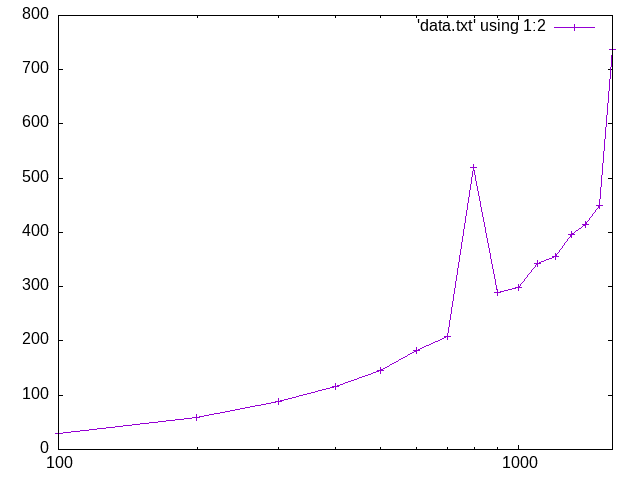
\includegraphics[width=0.8\textwidth]{plot.png}
    \caption{An example of a spike in the execution time.}
    \label{fig:1}
\end{figure}


As a result, my estimation was extremely close to the actual obtained result, which can be seen in the next section where it 
is also compared to sorted array's one. Given this situation, the sorted array is \textit{1.1} times slower than the unsorted one. 


\section*{Searching in a sorted array}

Here's the section where the interesting part I was talking about in the introduction comes in. Before creating the benchmark and running any code,
my wild guess was that: \textit{an extra condition to stop when the key is larger = significantly less time}. Well, is that the case all the time?

Moreover, as it can be noticed from the table below, the answer to the posed question is, 
therefore, no - an optimisation doesn't always make the algorithm faster, especially in certain situations: for instance 
if the element is not found at all or found, but close to the end of the sorted array. The \textbf{CoeffDiff} column refers to the 
absolute value as a result of the difference 
between the obtained and estimated coefficient. I decided to include this piece of information in the table as well since
after having run the code, I was impressed of how close the estimation actually was.

\begin{table}[h!]
    \centering
    \begin{tabular}{||c c c c c||} 
    \hline
    Type & ArraySize & EstimatedTime &  ObtainedTime & CoeffDiff\\ [0.5ex]
    Unsorted & $10^6$ & 0.44 & 0.48 & 0.04 \\
    Sorted & $10^6$ & 0.49 & 0.4 & 0.09\\ [1ex] 
    \hline
    \end{tabular}
    \caption{Comparison between the estimated and obtained coefficient.} 
    \label{table:1}
\end{table}

\begin{minted}{java}
                if(array[index] > key) {
                    return false;
                } 
\end{minted}


And apparently, the unexpected slowliness is because of the time that is lost, checking for each element the above new added condition
in order to optimise the algorithm. However, it should be noted that if the element is found,
this improvement does pay off timewise.

\subsection*{The Binary Search}

The binary search is an extremely efficient algorithm, since given a sorted array,
the space where the search for a specific key goes on is always diminished by half.
In other words, in terms of how efficient it is, the numbers speak for themselves as follows:

\begin{figure}[ht]
    \centering
    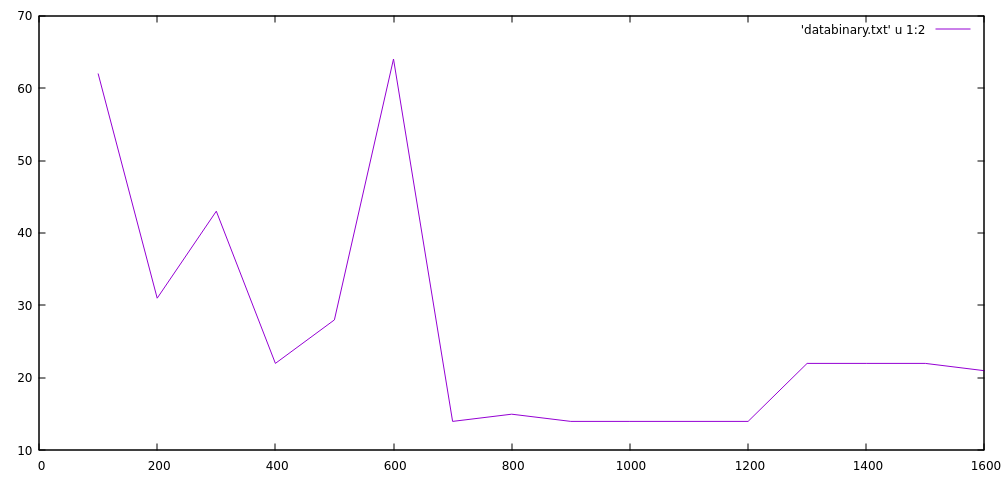
\includegraphics[width=0.8\textwidth]{plotbinary.png}
    \caption{The function describing the binary search execution time.}
    \label{fig:2}
\end{figure}

As far as the graph above is concerned, its relevant part is precisely where the almost linear parts are \textit{(starting 
on the x-axis with an array of 
700 elements)}, since it's there where we can 
notice the almost constant change when increasing the 
number of elements in an array and in other words, observe the logarithmic behaviour of the binary search. \newline \newline
On the other hand, the spikes are not of particular interest simply because we can not draw any conclusion.
And that is because of the high contrast between their peak value and the other ones. This contrast is most probably due to the fact that 
in the beginning, those values are not cached.


\begin{table}[h!]
    \centering
    \begin{tabular}{||c c ||} 
    \hline\hline
    n & LinBinRatio \\ [0.5ex]
    \hline
    100 & 6.4\\
    200 & 4.3\\
    400 & 9.1\\
    600& 5.7\\
    800 & 16.4\\
    1000 & 21.6\\
    1200 & 25.3 \\
    1400 & 19.0 \\
    1600 & 23.4 \\ [1ex] 
    \hline
    \end{tabular}
    \caption{The evolution of the ratio between the linear and binary search depending on the array's size.} 
    \label{table:2}
\end{table}

To put it briefly, the linear search in \textit{a sorted array} is much less efficient than the binary one and the obtained ratio between 
the two is proportional with the array's 
size. In other words, as the data set grows, so does it. To illustrate this, for an array of 1 million elements,
the linear search is \textbf{11363.7596} times slower than binary one. However, that is not it.
Turns out, the binary search becomes even more efficient as the array grows. For example, my timewise estimation for a 64 million long
array was \textbf{$58*10^3$} \textit{greater} than the actual result, which was highly impressive to say the least. 

\subsection*{Looking for duplicates} 

As discussed above, looking for duplicates in an unsorted array, will unddoubtedly be the most inefficient case  since it is an 
algorithm that goes under the category of \textit{O($n^2$)}.
That is precisely why, in this subsection, I decided to focus on the sorted arrays related experiments, which we assume do 
not contain duplicates themselves.

After having set up my code for the final, improved version described in the PDF, I noticed that, in order to look for duplicates,
the new algorithm, which uses two sorted arrays is \textbf{213} times better than the normal binary search for the given benchmark, therefore for an array
of maximum 1600 elements. \newpage

\begin{figure}[ht]
    \centering
    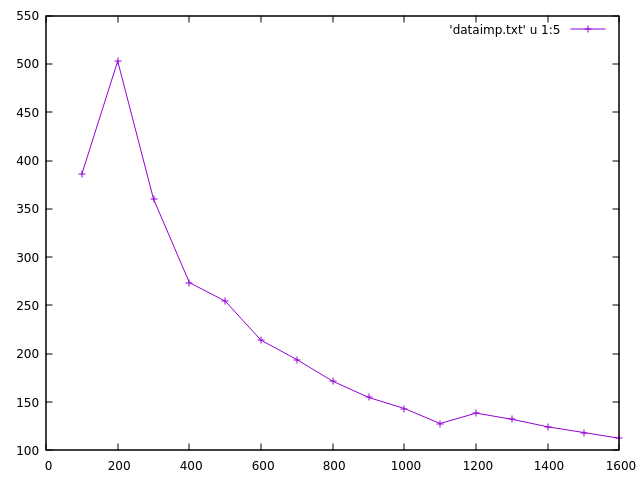
\includegraphics[width=0.8\textwidth]{plot_improved alg.png}
    \caption{The binary and improved version ratio evolution.}
    \label{fig:3}
\end{figure}

What's interesting about the evolution of the 
ratio between the binary search and the improved alternative
is that the ratio between the two
decreases, eventually \textit{tending towards 0} as the array increases. Take the case of an array of 1 million elements for example:

\begin{table}[h!]
    \centering
    \begin{tabular}{||c c c c||} 
    \hline\hline\newline
    Size & BinarySearchTime [ns] & ImprovedAlgTime [ns] & Ratio\\ [0.5ex]
    \hline
    $10^6$ & 151 & 787 & 0.1\\[1ex] 
    \hline
    \end{tabular}
    \caption{Time analysis for an array of 1 million elements.} 
    \label{table:3}
\end{table}

As a conclusion, in spite of the first impression, for large data sets, the binary search still remains the most efficient! 

\begin{minted}{java}
public static void better (int [] array, int [] index) {
    int j=-1, i=-1, count = 0;
    while (i < array.length -1 && j < index.length -1) {
    
        if(index[j+1] < array[i+1]) 
            j++;
        else {
            if (index[j+1] == array[i+1]) 
                count++;
            i++;
        }
}}
\end{minted}
    
\textit{Note: } I have included above, my code set up for the algorithm described in the assignment PDF.


\section*{Difficulties}

The main difficulty I have encountered in this assignment was related on how large should the set of the interval from where I generated the
random arrays and keys be. Had it been too small, the probability to have duplicates and therefore, not so relevant 
results for the time analysis would increase. In other words, I was not able 
to come up with a reliable depencency between time and the data set. After having drawn this conclusion, 
I, therefore, randomly populated an array and picked a key from an 
interval equal to the array's size.

\section*{Conclusion}
All in all, after having reached the end of this paper, numbers undoubtedly speak for temsselves. 
To put this in other words and in order to answer the last question of this 
experiment, operating on
sorted data sets is much more efficient than working on unsorted ones. However, how much does sorting cost in terms of 
resources will be elaborated in the next report!
\end{document}